
\documentclass[11pt]{article}
\usepackage[a4paper,margin=1in]{geometry}
\usepackage[T1]{fontenc}
\usepackage[utf8]{inputenc}
\usepackage{lmodern}
\usepackage{microtype}
\usepackage{amsmath,amssymb,amsfonts,bm}
\usepackage{graphicx}
\usepackage{booktabs}
\usepackage{float}
\usepackage{caption}
\usepackage{setspace}
\usepackage{hyperref}
\usepackage{enumitem}
\usepackage{array}
\usepackage{tabularx}
\usepackage{makecell}
\usepackage{mathtools}
\usepackage[numbers,sort&compress]{natbib}
\hypersetup{colorlinks=true, linkcolor=black, citecolor=black, urlcolor=blue}
\setstretch{1.08}
\setlength{\parskip}{0.45em}
\setlength{\parindent}{1.2em}
\captionsetup{font=small,labelfont=bf}
\graphicspath{{figures/}}
\sloppy
\emergencystretch=2em

\title{\vspace{-1.5em}\textbf{Socio-Traffic Thermodynamics:}\\[0.25em]
\large Integrated Model and Risk-Budgeted Information-Release\\[0.15em]
\large Audit Synthesis}
\author{Keiji Yoshimura\\\small Independent Researcher}
\date{May 25, 2026\\[0.35em]
\small Version: v0.3.1-integrated-revision-source-license-checked\\
\small GitHub repository: \href{https://github.com/yokken0907/socio-traffic-thermodynamics}{github.com/yokken0907/socio-traffic-thermodynamics}}

\begin{document}
\maketitle

\begin{abstract}
Socio-Traffic Thermodynamics (STT) is a claim-bounded theoretical and numerical framework for interpreting congestion recurrence as a non-equilibrium pattern generated by socially motivated motion on finite-capacity, finite-bandwidth transportation networks. The original manuscript introduced a mesoscopic formulation combining social potential, finite perceptual bandwidth, stochastic car-following dynamics, information compression, and dissipative stop-and-go wave formation in a periodic Optimal Velocity ring-road surrogate. The subsequent v0.2.0--v0.2.9 audit sequence narrowed and strengthened one operational subclaim: in finite-capacity toy networks, route information can reduce mean social cost only when it does not induce excessive synchronized reaction and overload severity. This v0.3.1 integrated revision combines the original model development with the later risk-budgeted information-release audits. The locked synthesis is conservative: risk-budgeted low-rate, coarse, staggered, or guarded information release reduced mean cost relative to a no-information null in the frozen holdout while not increasing overload severity, whereas common precise and delayed common information increased synchronization, overload, and cost. The manuscript does not claim real-world traffic prediction, traffic-policy validation, city-scale deployment readiness, or a universal congestion solution. It should be read as a hypothesis-generating toy-model synthesis about synchronization risk, information release, and buffering architecture under finite capacity.
\end{abstract}

\paragraph{Reader guidance and claim boundary.}
This manuscript is a claim-bounded integrated revision. The older STT formulation is retained as a model-building scaffold, while the v0.2.x audits restrict the positive claim to tested toy networks and frozen holdout designs. The work is adjacent to classical car-following instability, stop-and-go wave formation, traffic-flow theory, routing-game inefficiency, and information-design effects \cite{Bando1995,Sugiyama2008,Helbing2001,Roughgarden2003,Acemoglu2018,Das2017}. It is not a calibrated urban simulation, a route-guidance product, a traffic-policy recommendation, or a claim that congestion can be universally eliminated. The allowed claims concern finite-capacity toy networks, risk-budgeted information release, action synchronization, overload severity, and reduced surrogate diagnostics.

\section{Introduction}
Traffic congestion is often framed as an engineering inefficiency to be minimized by capacity expansion, signal control, route guidance, or demand management. That framing is useful but incomplete. Congestion can emerge endogenously even in the absence of an explicit bottleneck: fluctuations in an otherwise homogeneous stream can grow, destabilize free flow, and form backward-propagating jam waves once the system approaches a critical density or loses string stability \cite{Bando1995,Sugiyama2008,Helbing2001}.

Network-level routing adds another complication. Selfish routing can fail to minimize aggregate latency, as formalized by price-of-anarchy results \cite{Roughgarden2003}. More information is not automatically better: informational Braess-type effects can worsen aggregate outcomes when better-informed users react in correlated ways \cite{Acemoglu2018}, whereas carefully designed private or garbled signals can sometimes move equilibrium flows toward lower social cost \cite{Das2017}.

STT addresses this combined problem by treating congestion as a recurrent non-equilibrium structure on finite-bandwidth social-traffic networks. The present version does not expand this into a universal social theory. Instead, it integrates the original theoretical formulation with a later audit program that asks a narrower design question: when can information release improve mean efficiency without increasing overload risk relative to a conservative null?

\section{Model Formulation}
\subsection{Network and state variables}
Let $G=(V,E)$ be a directed transportation network. Let $\Omega$ denote a large finite or continuum population of agents. Each agent $i\in\Omega$ is characterized by position $x_i(t)$, velocity $v_i(t)$, internal state $s_i(t)\in[-1,1]$, route $p_i(t)\in\mathcal P$, and destination-dependent social potential $\Phi_i=\Phi(x_i,t)$.

Define macroscopic fields
\begin{equation}
\rho(x,t),\qquad u(x,t),\qquad m(x,t):=\mathbb E[s_i\mid x_i=x],
\end{equation}
where $\rho$ is density, $u$ is mean velocity, and $m$ is an order parameter representing local synchronization of internal states.

\subsection{Microscopic longitudinal dynamics}
For each agent,
\begin{equation}
\dot{x}_i=v_i,
\end{equation}
\begin{equation}
\dot{v}_i=F(h_i,\Delta v_i,s_i;\rho_i,\Phi_i)+\varepsilon_i(t)+\sqrt{2D_v}\,\xi_i(t),
\end{equation}
where $h_i$ is headway, $\Delta v_i$ is relative velocity, $F$ is a smooth car-following response, $\varepsilon_i(t)$ is decentralized residual control, and $\xi_i(t)$ is white noise.

The internal-state dynamics is modeled as
\begin{equation}
\tau_s\dot{s}_i=-s_i+\tanh\!\left(\beta[J(\mathcal K*s)_i+\lambda\Phi_i-\kappa C_i]\right)+\sqrt{2D_s^{\mathrm{eff}}}\,\zeta_i(t),
\end{equation}
with perceived congestion cost $C_i$ and effective internal noise
\begin{equation}
D_s^{\mathrm{eff}}=D_{s,0}+\chi_{\mathrm{sov}}\sigma_{\mathrm{sov}}^2+\chi_W W_i^{-1}.
\end{equation}
Here $W_i$ denotes effective perceptual bandwidth. The term $\sigma_{\mathrm{sov}}$ is not a normative judgment about individual freedom; it is a toy-model variance term representing decentralized residual control or idiosyncratic response.

\subsection{Route choice and information signal}
Given information $\mathcal I_i$, agent $i$ chooses a path $p\in\mathcal P$ with probability
\begin{equation}
\mathbb P(p_i=p\mid \mathcal I_i)=\frac{\exp\{-\theta[\mathcal C_p-\lambda_\Phi\Phi_p]\}}{\sum_{q\in\mathcal P}\exp\{-\theta[\mathcal C_q-\lambda_\Phi\Phi_q]\}},
\end{equation}
where $\mathcal C_p$ is generalized travel cost and $\Phi_p$ is destination-adjusted social potential. In the audit sequence, this formulation is specialized into finite-capacity route-choice toy networks with information policies ranging from no-information nulls to common precise, delayed common, coarse, staggered, guarded, and risk-budgeted releases.

\subsection{Macroscopic closure}
Under mean-field closure, a schematic macroscopic form is
\begin{equation}
\partial_t\rho+\nabla\!\cdot(\rho u)=0,
\end{equation}
\begin{equation}
\partial_t(\rho u)+\nabla\!\cdot(\rho u\otimes u)=-\nabla P(\rho,m)-\frac{\rho}{\tau}[u-U(\rho,m,\Phi)]+\nu\Delta u+\sqrt{2D_u\rho}\,\eta,
\end{equation}
\begin{equation}
\tau_m\partial_t m=A(\rho-\rho_c)m-Bm^3+D_m\Delta m+\lambda\Phi-\kappa C(\rho)-m+\sqrt{2D_m^{\mathrm{eff}}}\,\zeta.
\end{equation}
This closure is a conceptual reduced model. It is not asserted to be a calibrated continuum theory for any particular city.

\section{Metastability and Information Buffering}
\subsection{Metastability and jam nucleation}
Let $(\rho_0,u_0,m_0)$ be a homogeneous free-flow equilibrium. Fourier linearization yields
\begin{equation}
\dot{\hat z}_k=A_k\hat z_k+B_k\hat\omega_k+G_k\hat\xi_k.
\end{equation}
The system is linearly stable if $\Re\lambda(A_k)<0$ for all $k$. It is metastable if the stability margin
\begin{equation}
\alpha:=\min_k\{-\Re\lambda_{\max}(A_k)\}
\end{equation}
is positive but small. In that regime, perturbations decay slowly and rare transitions become more likely. Near a critical stop-and-go mode with amplitude $a$,
\begin{equation}
\dot{a}=-\partial_a\mathcal V(a;\rho,\Phi)+\sqrt{2D_{\mathrm{eff}}}\,\eta(t),
\end{equation}
with
\begin{equation}
D_{\mathrm{eff}}=D_0+\chi_{\mathrm{sov}}\sigma_{\mathrm{sov}}^2+\chi_W W^{-1}.
\end{equation}
The nucleation-rate heuristic
\begin{equation}
r_{\mathrm{nuc}}\asymp\exp\!\left[-\frac{\Delta\mathcal V(\rho,\Phi)}{D_{\mathrm{eff}}}\right]
\end{equation}
expresses the claim that systems near criticality become more vulnerable to fluctuation-driven jam formation.

\subsection{Variance principle for information buffering}
Let $X$ denote network state and $Y_i$ the signal received by agent $i$. A signal policy is a stochastic kernel $K(y\mid x)$. Path choices induced by $\{Y_i\}$ generate edge loads
\begin{equation}
F_e=\sum_{i=1}^{N}\mathbf 1\{e\in A_i\}.
\end{equation}
If edge social cost $SC_e(f)=fc_e(f)$ is convex, then
\begin{equation}
\mathbb E[SC(F)]=SC(\bar F)+\frac{1}{2}\sum_e SC_e''(\bar F_e)\,\mathrm{Var}(F_e)+o(\mathrm{Var}(F_e)),
\end{equation}
and
\begin{equation}
\mathrm{Var}(F_e)=\sum_i\mathrm{Var}(A_{ie})+2\sum_{i<j}\mathrm{Cov}(A_{ie},A_{je}).
\end{equation}
The key mechanism is therefore not information quantity alone but action covariance. Public high-resolution information can reduce uncertainty while increasing conditional action correlation. Coarse, private, staggered, or rate-limited information can preserve enough adaptation while suppressing synchronized load injection.

\section{Original Ring-Road Diagnostic}
\subsection{Simulation setting}
To test whether the STT transition mechanism appears in a minimal microscopic system, the original manuscript used a one-lane periodic ring with an Optimal Velocity (OV) car-following law \cite{Bando1995} and additive residual stochastic input:
\begin{equation}
\dot{x}_i=v_i,
\end{equation}
\begin{equation}
\dot{v}_i=a[V(h_i)-v_i]+\sigma_{\mathrm{sov}}\xi_i(t),
\end{equation}
where $h_i=x_{i+1}-x_i$ is headway on the ring and $\xi_i(t)$ is a zero-mean unit Gaussian process.

\subsection{Space-time observation}
Figure~\ref{fig:spacetime} shows the resulting space-time diagram. The trajectories begin near parallel, indicating approximate uniform flow. As the system evolves, localized bunching emerges and forms a persistent high-density band that propagates backward relative to vehicle motion. This is the canonical signature of a self-sustained stop-and-go wave \cite{Sugiyama2008}.

\begin{figure}[H]
\centering
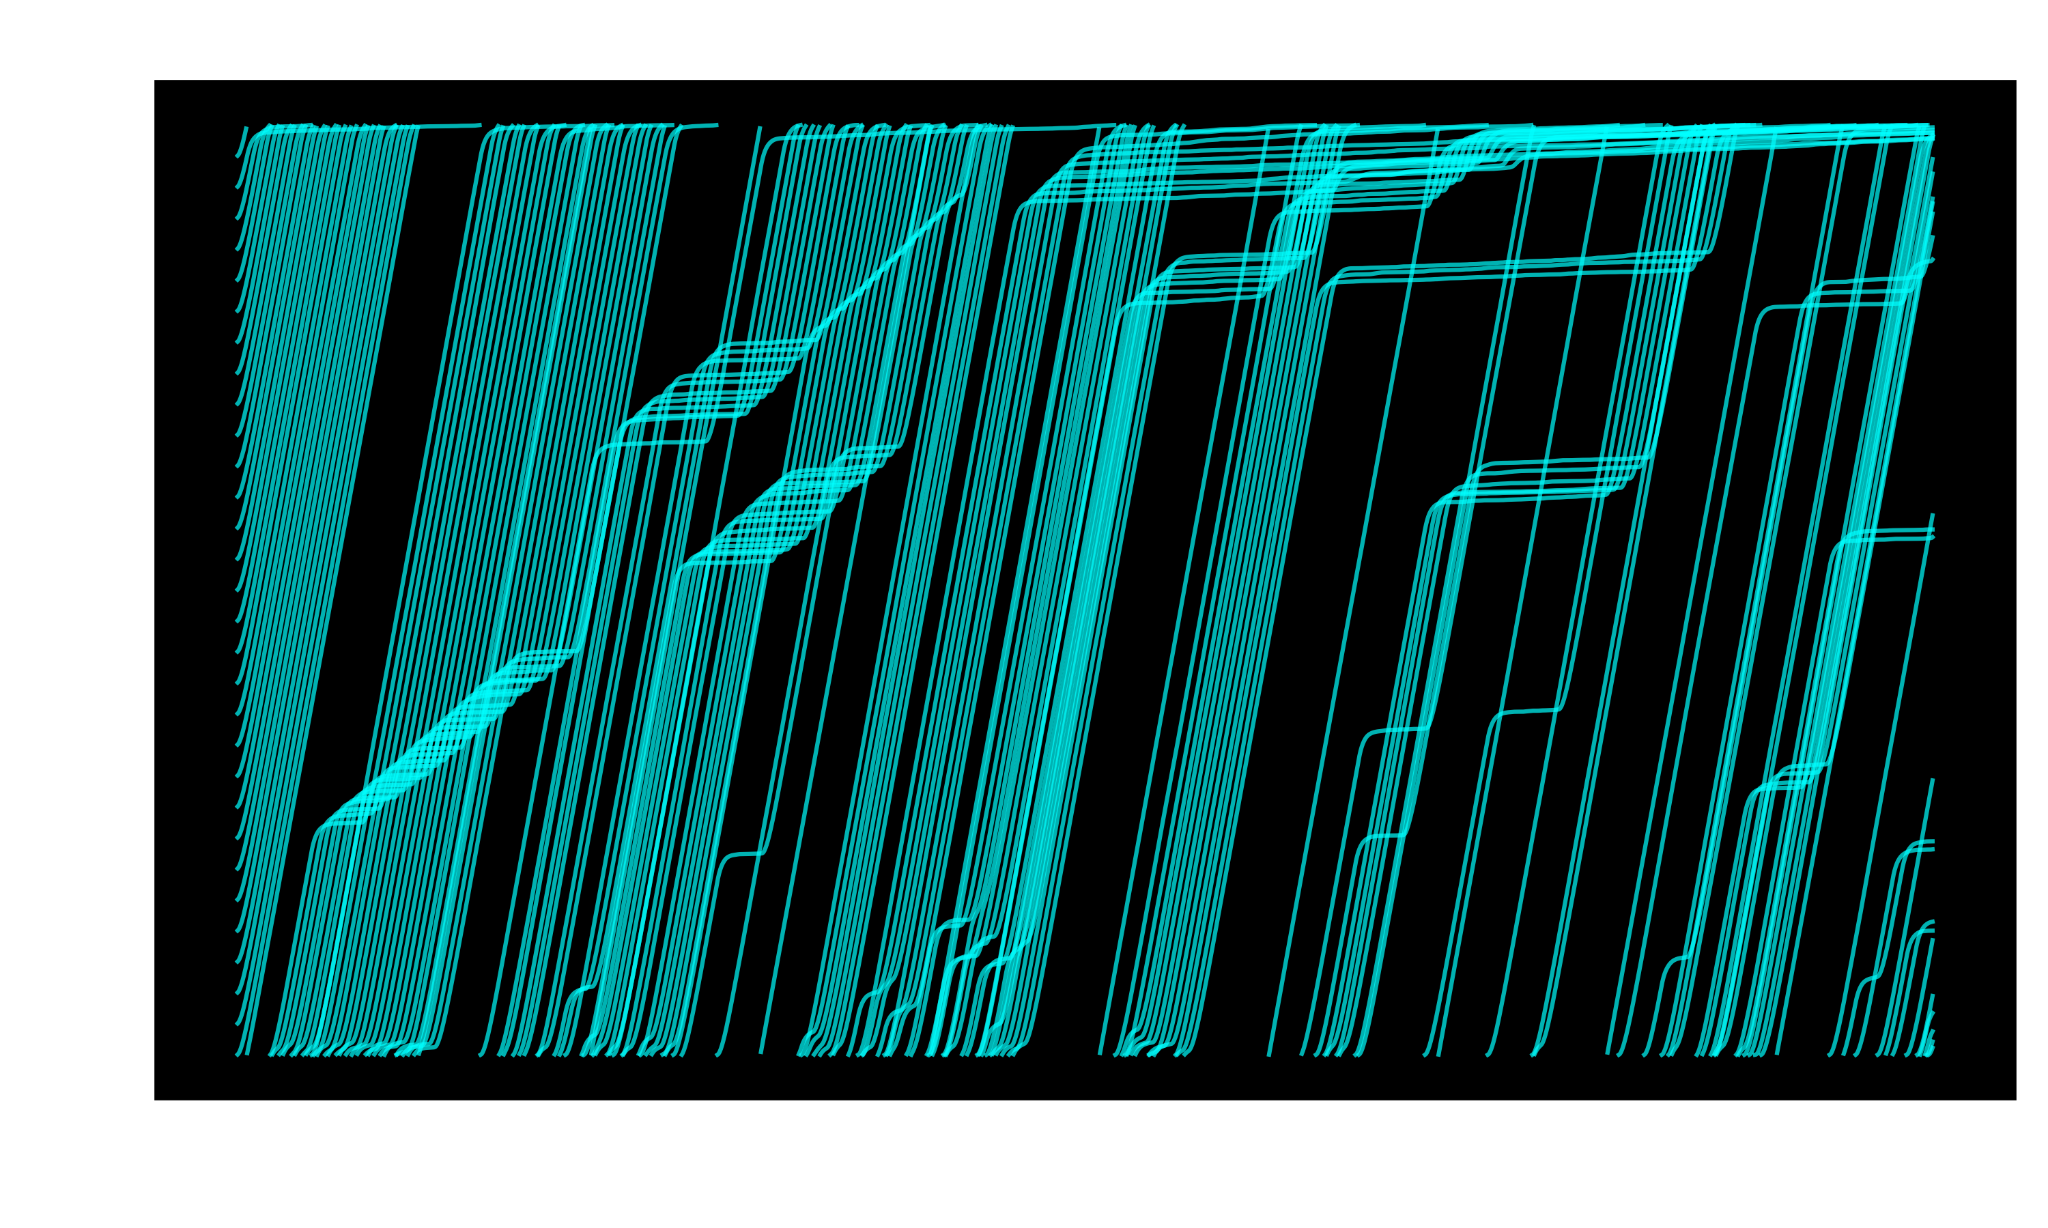
\includegraphics[width=0.96\linewidth]{stt_result.png}
\caption{Space-time diagram of the stochastic OV ring-road simulation. The figure is used as a minimal reduced diagnostic of endogenous stop-and-go wave formation, not as a calibrated city-scale traffic simulation.}
\label{fig:spacetime}
\end{figure}

\subsection{Dissipative-structure interpretation}
The backward-propagating wave is not interpreted as a conservative traveling mode. It is a dissipative structure sustained by throughput, relaxation delay, and irreversible adaptation. A schematic diagnostic is
\begin{equation}
\Sigma_{\mathrm{irr}}=\int_{\Omega_x}\left[\alpha_1|\partial_x u|^2+\alpha_2|\partial_t u|^2+\alpha_3\operatorname{Var}(u\mid x)\right]dx.
\end{equation}
The phrase ``dissipative structure'' is therefore used in an operationally bounded sense: it denotes an organized non-equilibrium pattern whose existence depends on ongoing flux and dissipation \cite{Helbing2001}.

\section{Risk-Budgeted Information-Release Audit}
\subsection{Audit program}
The v0.2.x program consisted of ten logged phases. Each phase preserved the toy-model boundary and avoided real-world policy interpretation.

\begin{table}[H]
\centering
\small
\caption{STT v0.2.x audit sequence. The status tokens are displayed in shortened form to avoid layout overclaiming and to keep the table readable.}
\begin{tabularx}{\linewidth}{p{0.14\linewidth}X p{0.24\linewidth}}
\toprule
Phase & Purpose & Status \\
\midrule
v0.2.0 & Phase diagram and information-buffering preflight & PASS preflight \\
v0.2.1 & Information-synchronization stress test & PASS run \\
v0.2.2 & Desynchronization audit & PASS run \\
v0.2.3 & Capacity-margin audit & PASS run \\
v0.2.4 & Buffer-architecture audit & PASS run \\
v0.2.5 & Mechanism-isolation audit & PASS run \\
v0.2.6 & Topology and demand robustness audit & PASS run \\
v0.2.7 & Risk-weighted Pareto audit & PASS run \\
v0.2.8 & Risk-budgeted information-release audit & PASS run \\
v0.2.9 & Frozen-policy holdout audit & PASS run \\
\bottomrule
\end{tabularx}
\end{table}

The terminal synthesis found all ten expected phase outputs and fixed the decision as the following synthesis-lock status:
\begin{center}
\small\ttfamily
PASS-STT-V030-\\
SYNTHESIS-LOCKED
\end{center}

\subsection{Risk-budget formulation}
Let $C$ denote mean social cost and $S$ denote overload severity. The no-information policy is used as a conservative null baseline with metrics $(C_0,S_0)$. A candidate information policy $\pi$ is admissible under severity budget $\epsilon_{\mathrm{sev}}$ if
\begin{equation}
S(\pi)-S_0\leq \epsilon_{\mathrm{sev}}.
\end{equation}
Among admissible policies, the design objective is
\begin{equation}
\Delta C(\pi)=C_0-C(\pi)>0.
\end{equation}
The strict zero-budget condition $\epsilon_{\mathrm{sev}}=0$ requires mean-cost improvement without increasing overload severity relative to the no-information null.

\subsection{Frozen holdout results}
The v0.2.9 audit froze candidate policy families from prior phases and evaluated them on holdout topologies, pulse modes, utilizations, and seeds.

\begin{table}[H]
\centering
\small
\caption{Representative v0.2.9 frozen-holdout policy results. Positive improvement means lower mean cost than the no-information baseline.}
\begin{tabularx}{\linewidth}{X r r r r}
\toprule
Policy & Mean cost & Severity & Sync & Improvement \\
\midrule
budget\_common\_u0.055\_s0.00 & 1.734 & 0.0227 & 0.0028 & 0.024 \\
budget\_common\_u0.035\_s0.00 & 1.734 & 0.0228 & 0.0019 & 0.024 \\
coarse\_zone\_u0.035 & 1.736 & 0.0228 & 0.0041 & 0.023 \\
staggered\_private\_u0.035 & 1.735 & 0.0228 & 0.0069 & 0.024 \\
no\_info & 1.759 & 0.0268 & 0.0000 & 0.000 \\
common\_precise & 3.568 & 0.2177 & 0.9244 & -1.809 \\
delayed\_common & 6.716 & 0.4381 & 0.9391 & -4.957 \\
\bottomrule
\end{tabularx}
\end{table}

The best mean-cost frozen policy was \texttt{budget\_common\_u0.055\_s0.00}. Its mean cost was 1.734372 compared with 1.758804 for no information, giving an improvement of 0.024432. Its overload severity was 0.022745, which was 0.004088 lower than the no-information baseline. By contrast, common precise and delayed common information substantially increased synchronization, overload, and cost.

\begin{figure}[H]
\centering
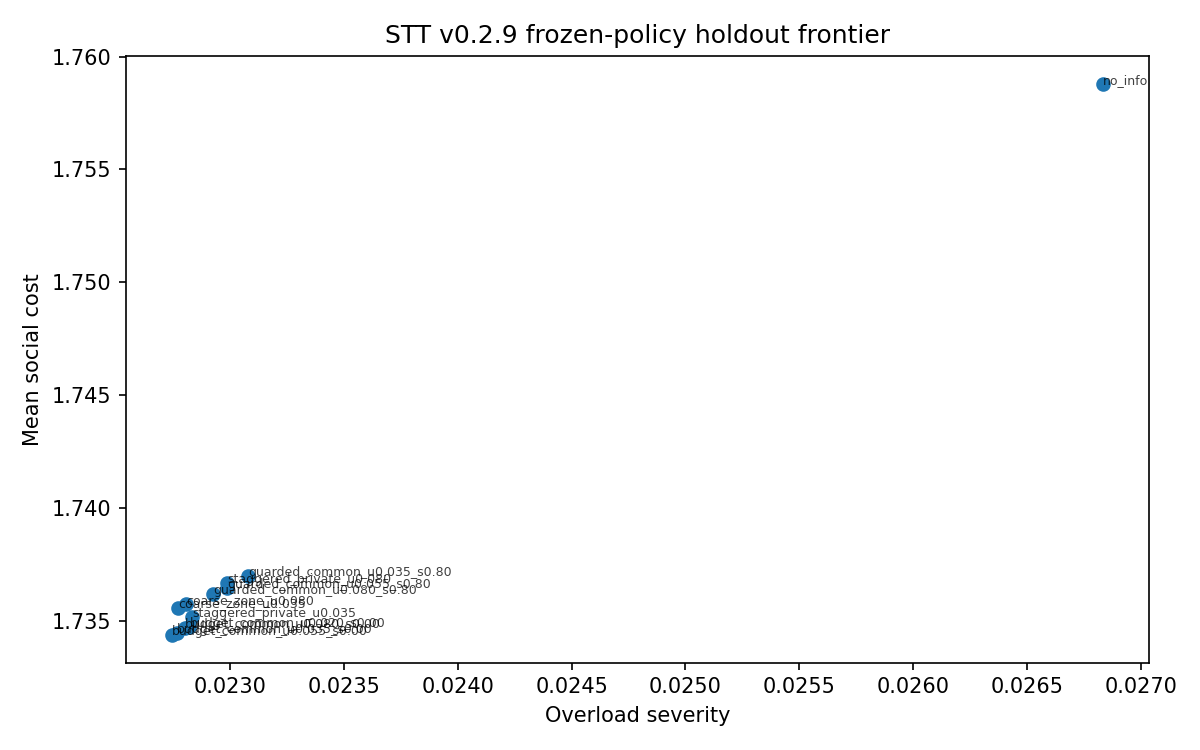
\includegraphics[width=0.86\linewidth]{stt_v029_holdout_frontier.png}
\caption{Frozen-policy holdout frontier from STT v0.2.9. Candidate risk-budgeted policies lie close to the lower-left region, while the no-information baseline is conservative but slightly less efficient.}
\label{fig:frontier}
\end{figure}

\subsection{Zero-budget finding}
Under the strict zero-budget condition, all 27 holdout conditions had at least one policy that improved mean cost without increasing overload severity relative to no information. The winning families were \texttt{budget\_common} and \texttt{coarse\_zone}.

\begin{table}[H]
\centering
\small
\caption{Zero-budget holdout winners.}
\begin{tabular}{lrrrr}
\toprule
Winner family & Win count & Win fraction & Mean improvement & Mean sync index \\
\midrule
budget\_common & 20 & 0.741 & 0.0273 & 0.0039 \\
coarse\_zone & 7 & 0.259 & 0.0176 & 0.0040 \\
\bottomrule
\end{tabular}
\end{table}

\begin{figure}[H]
\centering
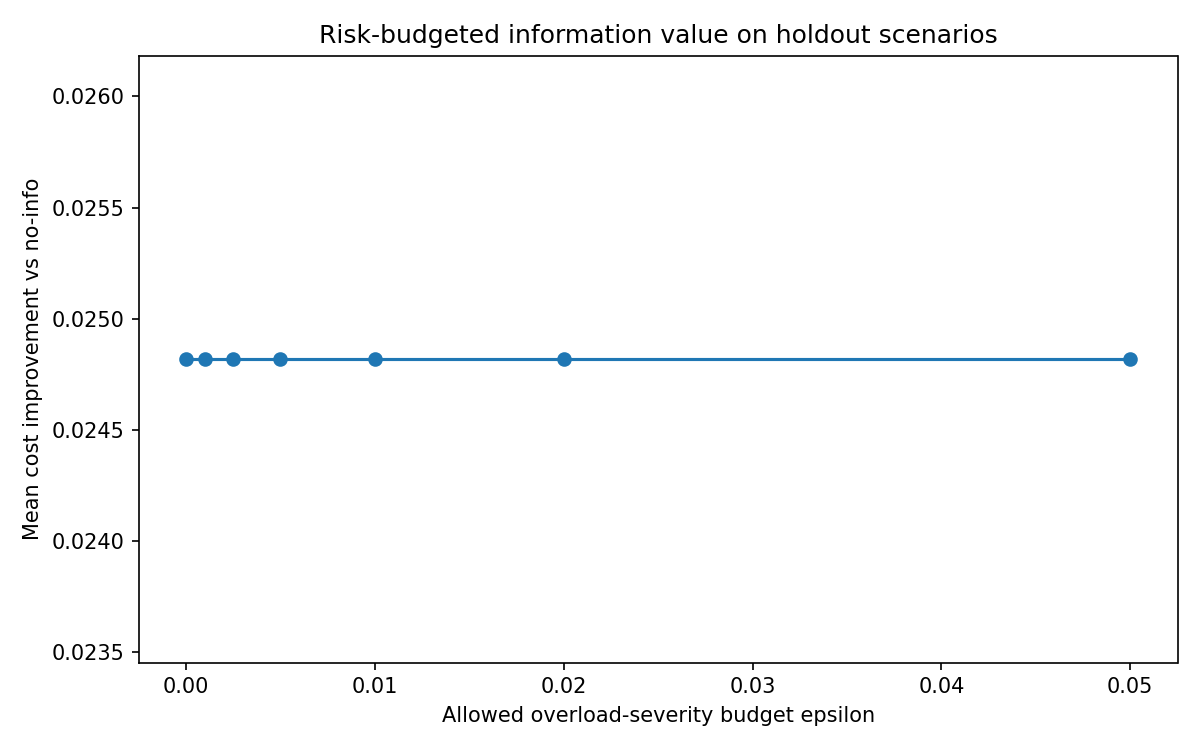
\includegraphics[width=0.82\linewidth]{stt_v029_budget_value_curve.png}
\caption{Risk-budgeted information value in the frozen holdout. In this holdout, the best available candidate already improves mean cost at zero additional overload-severity budget. The flat curve is a property of the tested candidate set and holdout design, not a universal traffic-policy claim.}
\label{fig:valuecurve}
\end{figure}

\section{Architectural Interpretation}
The integrated result narrows the original architectural interpretation. STT does not imply that all information should be restricted, nor that high-precision information is intrinsically harmful. The observed mechanism is synchronization risk under finite capacity. Shared precise information can reduce individual uncertainty while increasing conditional action correlation. If many agents respond in the same direction at the same time, finite-capacity links can be pushed into overload.

This suggests four buffering directions, each still at the hypothesis-generating level:
\begin{enumerate}[leftmargin=*]
\item \textbf{Temporal buffering:} reduce abrupt synchronization gradients rather than only lowering average demand.
\item \textbf{Spatial buffering:} use transfer basins, reservoirs, or staging regions to reduce sudden injection into metastable corridors.
\item \textbf{Informational buffering:} treat routing guidance as a variance-control channel rather than a universal shortest-path oracle.
\item \textbf{Behavioral buffering:} use damping-capable agents or protocols to reduce oscillatory amplification.
\end{enumerate}

\section{Limitations}
The strongest limitation is model class. The ring-road simulation is a minimal stochastic OV surrogate. The v0.2.x network audits are toy networks, not calibrated urban simulations. The policies are algorithmic abstractions rather than deployable route-guidance mechanisms. The metrics do not include equity, compliance heterogeneity, public trust, legal constraints, safety, multimodal behavior, or real sensor latency. Therefore, the result is a hypothesis-generating diagnostic claim rather than an operational traffic-policy claim.

A second limitation is baseline definition. The no-information baseline is conservative in this toy design, whereas real systems already contain heterogeneous information sources, institutional controls, learned route preferences, and external routing platforms. Any empirical extension must define the baseline carefully.

\section{Next Validation Tier}
The next validation tier should not be another small toy audit. It should use externally defined synthetic networks or public benchmark traffic scenarios with frozen candidate policies and predeclared metrics. The minimum extension should preserve: (i) a no-information or status-quo baseline, (ii) an overload-risk metric, (iii) a mean-efficiency metric, (iv) a synchronization metric, and (v) a frozen holdout protocol.

\section{Conclusion}
The integrated STT result is narrower but stronger than the original broad framing. Congestion can be modeled as a non-equilibrium dissipative pattern in socially attractive, finite-capacity networks, and the original ring-road surrogate illustrates endogenous stop-and-go wave formation without a fixed bottleneck. The later risk-budgeted audit adds a more operational lesson: in finite-capacity toy networks, information release should be treated as a synchronization-control problem under overload-risk constraints, not merely as a route-precision maximization problem.

\section*{Data and Code Availability}
The manuscript is accompanied by a repository package containing the integrated manuscript source, selected figures, original ring-road scripts, v0.3.0 synthesis outputs, manifest files, claim-boundary documentation, and source-defined evaluation-only license files. The GitHub repository is available at \href{https://github.com/yokken0907/socio-traffic-thermodynamics}{github.com/yokken0907/socio-traffic-thermodynamics}. Any future GitHub-Zenodo archive should be generated automatically from the release rather than manually assigning an external identifier.

\section*{Acknowledgments}
The author conceptually directed the theory-development and validation workflow. Large language models were used as computational, drafting, and software-assistance tools under direct human supervision. All claim-boundary decisions and release decisions remain the author's responsibility.

\begin{thebibliography}{99}
\bibitem{Bando1995} M. Bando, K. Hasebe, A. Nakayama, A. Shibata, and Y. Sugiyama, ``Dynamical model of traffic congestion and numerical simulation,'' \emph{Physical Review E} \textbf{51}, 1035--1042 (1995).
\bibitem{Sugiyama2008} Y. Sugiyama, M. Fukui, M. Kikuchi, K. Hasebe, A. Nakayama, K. Nishinari, S.-i. Tadaki, and S. Yukawa, ``Traffic jams without bottlenecks---experimental evidence for the physical mechanism of the formation of a jam,'' \emph{New Journal of Physics} \textbf{10}, 033001 (2008).
\bibitem{Helbing2001} D. Helbing, ``Traffic and related self-driven many-particle systems,'' \emph{Reviews of Modern Physics} \textbf{73}, 1067--1141 (2001).
\bibitem{Roughgarden2003} T. Roughgarden, ``The price of anarchy is independent of the network topology,'' \emph{Journal of Computer and System Sciences} \textbf{67}(2), 341--364 (2003).
\bibitem{Acemoglu2018} D. Acemoglu, A. Makhdoumi, A. Malekian, and A. Ozdaglar, ``Informational Braess' paradox: The effect of information on traffic congestion,'' \emph{Operations Research} \textbf{66}(4), 893--917 (2018).
\bibitem{Das2017} S. Das, E. Kamenica, and R. Mirka, ``Reducing congestion through information design,'' working paper (2017).
\end{thebibliography}
\end{document}
